\documentclass[journal,10pt,twocolumn]{article}
\usepackage{graphicx}
\usepackage[margin=0.5in]{geometry}
\usepackage{amsmath}
\usepackage{array}
\usepackage{booktabs}
\usepackage{amssymb}
\title{\textbf{Matrix Assignment}}
\author{lakshmi kamakshi}
\date{September 2022}

\begin{document}

\maketitle
\paragraph{\textit{Problem Statement} -ABCD is a rectangle and P, Q, R and S are mid-points of the sides AB, BC, CD and DA
respectively. Show that the quadrilateral PQRS is a rhombus.}
\vspace{5mm}

\section*{Solution}

Using triangle law of vector addition:
\begin{equation}
	\overline{PQ}= \overline{PB} + \overline{BQ} 
\end{equation}
\begin{equation}
		  \overline{PQ}  = \frac{1}{2}\overline{AB} + \frac{1}{2}\overline{BC} \\
\end{equation}
\begin{equation}
	\overline{PQ} =\frac{1}{2}(\overline{AB+BC})\\
\end{equation}
\begin{equation}
	  \overline{PQ} =\frac{1}{2}\overline{AC} \\
\end{equation}

Similarily,using triangle law of vector addition:
\begin{equation}
	\overline{PS}= \overline{PA} + \overline{AS} 
\end{equation}
\begin{equation}
		  \overline{PS}  = \frac{1}{2}\overline{BA} + \frac{1}{2}\overline{AD} \\
\end{equation}
\begin{equation}
	\overline{PS} =\frac{1}{2}(\overline{BA+AD})\\
\end{equation}
\begin{equation}
	  \overline{PS} =\frac{1}{2}\overline{BD} \\
\end{equation}
\\ABCD is a rectangle and has the following properties:
\begin{enumerate}
	\item Opposite sides are equal
\item All angles are equal
\item lengths of diagonals are equal
\item Diagonals are perpendicular to each other.
\end{enumerate}
	\begin{equation}
AC = BD 
	\end{equation}
	\begin{equation}
		AC \perp BD
	\end{equation}
	\begin{equation}
		\boldsymbol{PQ} = \boldsymbol{PS}
	\end{equation}
\\ similarly, the vector equations of QR,SR can be derived as:
\begin{equation}
	\overline{QR}= \overline{QC} + \overline{CR} 
\end{equation}
	
\begin{equation}
		  \overline{QR}  = \frac{1}{2}\overline{BC} + \frac{1}{2}\overline{CD} \\
\end{equation}
\begin{equation}
	\overline{PQ} =\frac{1}{2}(\overline{BC+CD})\\
\end{equation}
\begin{equation}
	  \overline{PQ} =\frac{1}{2}\overline{BD} \\
\end{equation}


\begin{equation}
	\overline{SR}= \overline{SD} + \overline{DR} 
\end{equation}
\begin{equation}
		  \overline{SR}  = \frac{1}{2}\overline{AD} + \frac{1}{2}\overline{DC} \\
\end{equation}
\begin{equation}
	\overline{SR} = \frac{1}{2}(\overline{AD}+\overline{DC})
\end{equation}
\begin{equation}
	\overline{SR} = \frac{1}{2}\overline{AC}
\end{equation}
from the equations (),():
\begin{equation}
	SR = QS
\end{equation}
\\ Thus, all sides of the quadrilateral PQRS are equal
\\ The diagonals of the Quadrilateral PQRS are given by:
\begin{equation}
	PR = PS+PQ
	\because
\end{equation}
parallelogram law of addition
\begin{equation}
	QS = PS-PQ
	\because
\end{equation}
triangle law of addition
\\ \begin{equation}
	PR = \frac{1}{2}\overline{AC}+\frac{1}{2}\overline{BD}
\end{equation}
\\ \begin{equation}
        QS = \frac{1}{2}\overline{AC}-\frac{1}{2}\overline{BD}
\end{equation}
\\ For a quadrilateral to be rhombus the diagonals should perpendicularly bisect each other
\begin{equation}
	PR.QS = \frac{1}{4}((\overline{AC}+\overline{BD})(\overline{AC}-\overline{BD}))
\end{equation}
\begin{equation}
	PR.QS = 0
\end{equation}
\\Since the dot product of the diagonals is 0, the diagonals are perpendicular
\section*{Construction}
Since , all sides of the qudarilateral PQRS are equal and the digonals are perpendicular to each other, the Quadrilateral is a Rhombus
\begin{figure}[h]
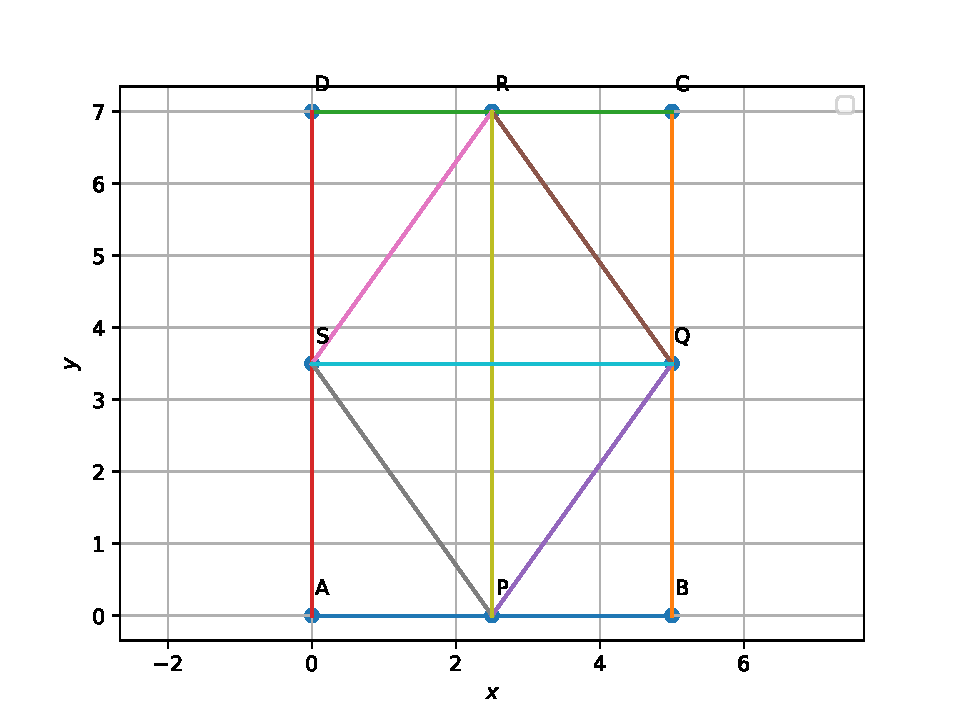
\includegraphics[width=1\columnwidth]{fig.pdf}
\caption{Rhombus PQRS formed by midpoints of Rectangle ABCD}
\end{figure}



\section*{Construction}
The dimensions of the rectangle are taken as below\\
{
\setlength\extrarowheight{2pt}
\centering
	\begin{tabular}{|c|c|}
	\hline
	\textbf{vertex}&\textbf{co-ordinates}\\
	\hline
	A&(0,0)\\
	\hline
	B&(5,0)\\
	\hline
	C&(5,7)\\
	\hline
	D&(0,7)\\
	\hline
\end{tabular}
}
\end{document}
